\chapter{Modeling}
\chapter{About Epithelial Tissue?}
Epithelial tissue covers the interior and exterior surfaces of our bodies. Skin, the lining of the esophogas and intestines, the urethra, the lining of the lungs and all of the bronchioles in the lungs are all made up of epithelial tissue. In this way, we can think of epithelial tissue as being the envelope in which our contents are packaged \cite{Shape Formation}; epithelial tissue is our interface with the outside world. 

\begin{figure}[hb]
\centering 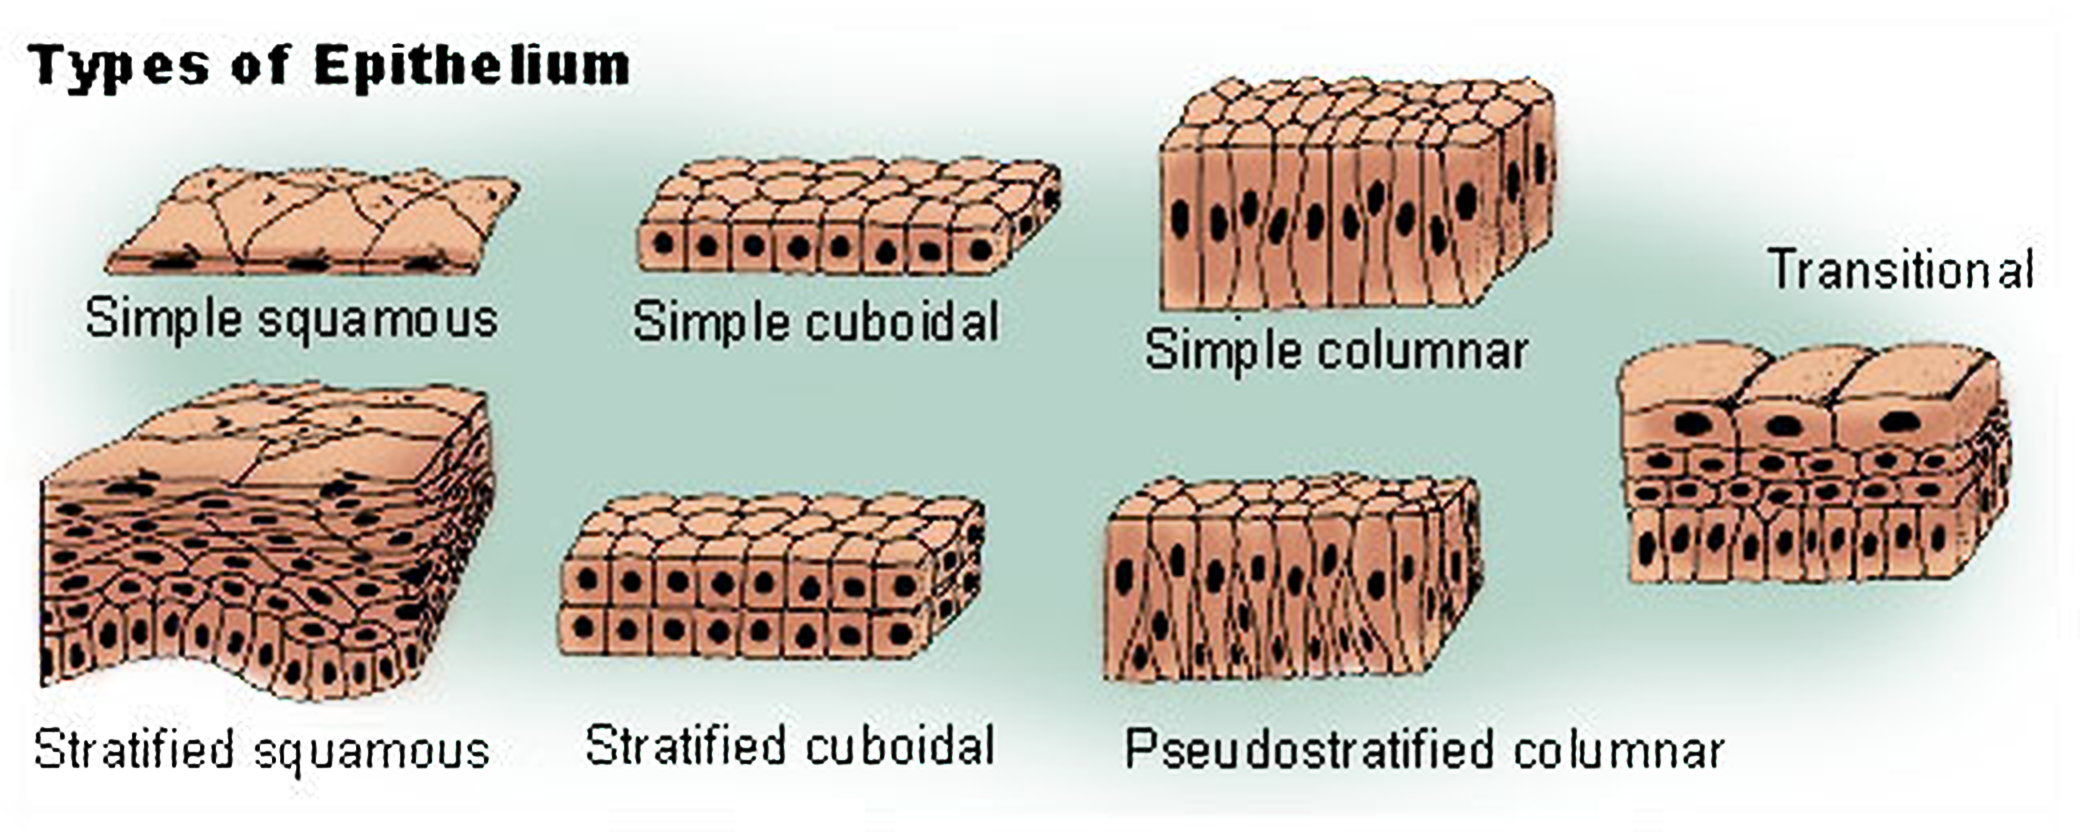
\includegraphics[width=\textwidth]{../diagrams/output.png}
\caption{The Types of Epithelial Tissue}
\label{fig:types}
\end{figure}

As Figure~\ref{fig:types} shows, there are many types of epithelial tissue in animals which vary in their number of layers and how the cells are shaped. Each of these types of cells are found in a different region of the body where they perform a specific function.  For example, the simple squamous epithelium is no more than one layer of cells thick, and the cells are all very flat, much flatter than they are wide. These cells are therefore well suited to  allow diffussion across themselves. As such, simple squamous tissue is found in the walls of blood vessels and in the alveoli in the lungs, where the diffusion of oxygen occurs. On the other hand, columnar cells are much taller than they are wide, and are thus well suited to absorption. These cells are found in the intestines where they absorb nutrients from passing food. Stratified squamous epithelia are several layers thick line the esophogas and mouth and serve to protect against abraision.

What all of these tissues have in common, however, is how amenable they are to computational modeling. The simplest case is that of simple epithelia, which typically have near-uniform height, and very little difference in appearance between their apical and basal faces. This means that the cells can easily be approximated by a two dimensional mesh, since the top and bottom of the cells move in tandem and the surface where two cells touch can be approximated by a line. See Figures CITE FIGURES HERE to see examples of current 2D models.  Slightly more difficult is the modeling of stratified tissue. In this case, the tissue develops in three dimensions, since underlying cells affect the cells on top of them CITE OKUDA IMAGE FOLLOWING DR. OVERMANS HELP WITH IMAGE FORMATTING. These cannot be modeled in two dimensions, but can be modeled by a solid composed of three dimensional polytopes. The theory behind these models is well developed, but the techincal details of implementing such a model has made it so that very exist, and are often quite limited \footnote{Even a leading epithelial tissue simulator, Chaste, still does not have stable 3D modeling capabilities}. For an example of a 3D model, see image INSERT IMAGE NAME HERE.

\begin{figure}[h]
    \centering
    \begin{subfigure}[b]{0.4\textwidth}
		\centering
		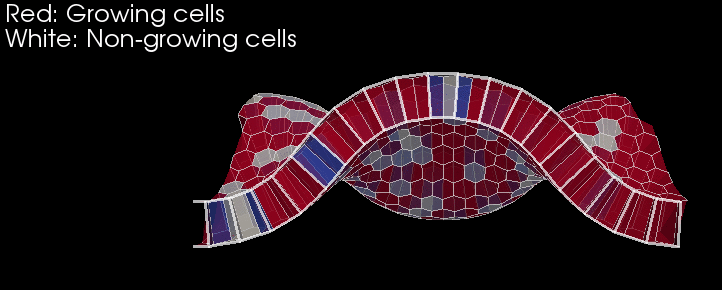
\includegraphics[width=\textwidth]{../diagrams/okuda1.png}
		\caption{Simple Squamous Tissue Bending in 3D\cite{Okuda1}}
		\label{fig:okuda1}
    \end{subfigure}
    \hfill
    \begin{subfigure}[b]{0.4\textwidth}
		\centering
		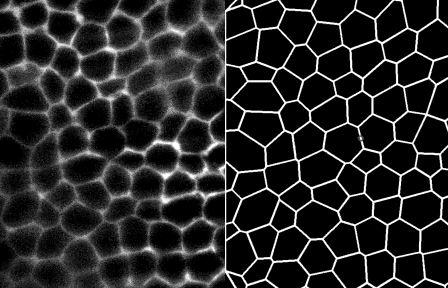
\includegraphics[width=\textwidth]{../diagrams/perfect.png}
		\caption{Comparison of Living Tissue and Simulation\cite{Yoshi}}
		\label{fig:yoshi}
    \end{subfigure}
    \hfill
    \begin{subfigure}[b]{0.4\textwidth}
        \centering
        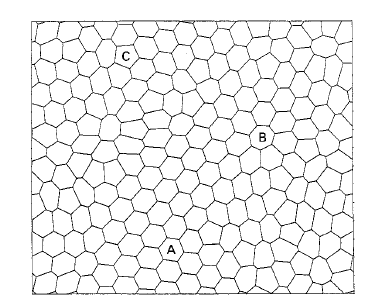
\includegraphics[width=\textwidth]{../diagrams/HondaResult.png}
        \caption{Equilibrium Mesh\cite{HondaNagai}}
        \label{fig:Honda}
    \end{subfigure}
    \hfill
    \begin{subfigure}[b]{0.4\textwidth}
        \centering
        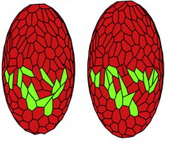
\includegraphics[width=\textwidth]{../diagrams/mirim.png}
        \caption{Equilibrium Mesh on a 3d Surface \cite{Vertex Models}}
        \label{fig:mirim}
    \end{subfigure}
    \caption{Some existing models of epithelial tissue.}
    \label{fig:four graphs}
\end{figure}


Current modeling is producing great results in the field of epithelial tissue morphogenisis, equilibration, and wound healing. The Honda-Nagai model which we will discuss in great detail in this paper successfully reproduced the wound healing of cats' corneas\cite{Wound Healing}. This model has also been able to reproduce all of the essential dynamics of epithelial tissue \cite{HondaNagai}. MENTION THE DROSOPHILA RESULTS. Current imaging tools have enabled the recording of epithelial tissue dynamics \emph{in vivo} CITE KIEHART AND MAGASON, providing a wealth of experimental data which can serve as either initial conditions for simulations, or as benchmarks to measure the success of computational models. In turn, models of epithelial dynamics can provide insights into the physical parameters that govern tissue development, maintenance, and illness.

Other modeling communities share advanced, free, and parallel simulation codes. For example, consider LAMMPS for simulating atomistic materials, and CHARMM, Amber,and NAMD for the molecular dynamics of biomolecules. Unfortunately, there are only a handful of codes in use for the simulation of ET, and only one of them is freely available \cite{ChasteMain}. In this thesis I will present the basic ideas of \textbf{vertex dynamics models}, and then describe the implementation of one of them in a freely available modeling tool for the community.

\section{Modeling Epithelial Tissue}
\begin{center}
\emph{The world was so recent that many things still lacked names,}\\
\emph{and to mention them one had to point with a finger. }\\
\textbf{\hspace{10ex} - Gabriel Garcia Marquez}
\end{center}
A two dimensional \textbf{vertex dynamics model} of epithelial tissue is made up of vertices and edges. A cell is represented as a convex hull made up of cells and vertices. This model presupposes that the movement of cells in epithelial tissue can be approximated by the movement of the vertices which make up the cell. Some force is hypothesized to be the guiding force between epithelial cell movement, and this force is applied to all of the vertices in the mesh of cells, producing some final state of the tissue. The three dimensional model is an extension of the two-dimensional model, but the mesh comes to include not only vertices and edges, but also cell faces. 

Epithelial vertex dynamics has been a lively field of research since the 1970s because of several heartening results in the field. Some researchers have had success modelling the morphogenesis of \emph{Drosophila} wing growth, whereas other researchers have successfully reproduced the dynamics of corneal wound healing. Unfortunately, these results have not come from one standard force, but from a variety of different hypothesized forces.

As an example of the different approaches to force modelling, let us consider the Weliky-Oster and Honda-Nagai forces. The Weliky-Oster model specifies explicit forces which act act upon the vertices due to a tension associated with boundary lengths. In two dimensions this constributes two tensions from each edge in a cell surrounding a vertex. The model also includes a cortical pressure due to the osmotic pressure inside a cell, which tends to push a vertex away from the interior. The Honda-Nagai Model (which I have recreated) takes a much different approach and instead specifies a potential energy function for the tissue. In this model the cells move passively as they attempt to minimize the potential energy of the tissue\cite{Vertex Models}. 

While both of these models successfully reproduce the topological and geometric properties of epithelial tissue, I have chosen to focus my efforts on the Nagai-Honda model. So, let us look at the model in some depth.

\section{The Nagai-Honda Model}
\subsection{How the Vertices Move}
A very basic result from physics is the relationship between force and potential energy, and this is one of the building blocks of the Nagai-Honda Model. Given a force vector $F$ and scalars $U$, for potential energy and $W$ for work, we can derive the relation:

\begin{gather}
\vec{F} = (F_x, F_y, F_z)\\
W = -\Delta U(\vec{x}) = \int_{x_0}^xF_xdx+\int_{y_0}^yF_ydy+\int_{z_0}^zF_zdz\\
\nabla(-\Delta U(\vec{x}) = \nabla\Bigg(\int_{x_0}^xF_xdx+\int_{y_0}^yF_ydy+\int_{z_0}^zF_zdz\Bigg)\\
-\nabla U(\vec{x}) = \vec{F}
\end{gather}

The second building block of the Nagai-Honda Model is the equation of motion. In 1989, K. Kawaski showed that the dynamics of grain growth can be reduced to a first order system given by:
\begin{equation}
\eta\frac{dr_i}{dt} = F_i
\end{equation}

where $F_i$ denotes the force applied to vertex $i$ and the left hand side is the velocity of the vertex multiplied by a positive drag coefficient, $\eta$\cite{1989 Kawasaki}.

\begin{figure}
\centering
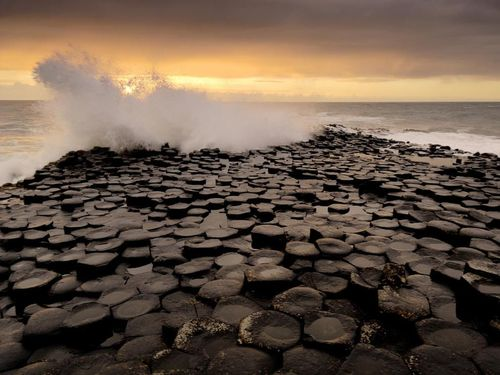
\includegraphics[width=0.5\textwidth]{../diagrams/resize_giant.jpg}
\caption{The Giant's Causeway}
\label{fig:cause}
\end{figure}

A very important paper in the field of natural cellular structures, of which the study of epithelial tissue is a small subset, is \emph{Soap, Cells, and Statistics}. In this paper, leading researchers in the field  argue that there must be some natural mechanism underlying the development of epithelial tissue, columnar basalt formations, soap froths, grin growths, and other cellular structures, as they exhibit a great deal of similarity. For example, consider the images of epithelial tissue presented throughout this paper next to the image of The Giant's Causeway in Northern Ireland. Some differences include the exact distribution of cell shapes, the presence of chemicals in biological tissues versus the absence of growth inducing chemicals in geological structures, and the active migration of biological cells versus the entirely passive movement of soap froths; still, the equilibrium patterns of these diverse structures leads one to believe that there must be some underlying principle. The Honda-Nagai model builds upon this idea and borrows ideas from the field of grain growth.

Putting these building blocks together, we have a force acting on the vertices in the mesh, and an equation of motion which explains how the vertices move. Now all that is needed is a free energy function from which to derive our force (and this force should be similar to the force found in other cellular structures). The free energy function which provides the applied force was taken in part from the grain growth model, which asserts that grains want to achieve a target volume and perimeter via some still unknown mechanism. As previously mentioned, biological cellls have idiosynchratic mechanisms working on them as well. As such, the model was extended to include a purely biological factor, \emph{differential adhesion}. It is well known that cells have a proclivity to attach more tightly to certain cells  than to others due to the presence of certain cadherin proteins in the membranes of the cells. This tendency is called differential adhesion.

The first two energy terms assume that the cell is elastic, and that the cell wants to return to a target shape. Therefore, the first two energy terms are of the elastic potential form: 
\begin{equation}
C(x-x_0)^2
\end{equation}
\begin{figure}
\centering
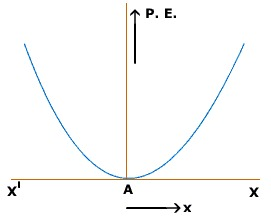
\includegraphics{../diagrams/pe.jpg}
\caption{Potential Energy as a Function of Distance from Equilibrium.}
\label{fig:pe}
\end{figure}
where $x$ is some physical quantity, and $C$ is some constant. The plot of this energy is therefore a parabola with a minimum at $x =  x_0$ ($A$ replaces $x_0$ in Figure~\ref{fig:pe}) and the farther $x$ is from $x_0$, the more potential energy there will be in the cell. 
The last energy term is an adhesion energy, which is proportional to the amount of interfacial surface area between a cell and its neighbor. Here are the three energy terms:
\begin{enumerate}
\item The deformation energy term \\ 
\begin{equation}
U_D = \lambda(A - A_0)^2
\end{equation}
 where $A_0$ is a target area for a cell, and lambda is some positive constant.
\item The membrane surface energy 
\begin{equation}
U_S = \beta(C - C_0)^2
\end{equation}
 where $C$ is the cell perimiter, and $C_0$ is a target perimeter.
\item The cell-cell adhesion energy 
\begin{equation}U_A = \displaystyle\sum\limits_{j = 1}^{n}\gamma_{j}d_{j}\end{equation}
where $n$ is the number of vertices in the cell, $\gamma$ is some constant for the boundary in question between one cell and another, and d is the distance between one vertex and the next in a counter clockwise fashion. Note that in two dimensins the boundary is a distance $d$, but in three dimensions it would have to be the area of a cell face. Also take note of the fact that the gamma term could be implemented in various ways. I have chosen to assign a ``stickiness'' to each cell, and then the gamma term is calculated as the average of the stickiness of the two cells.
\end{enumerate}

 As seen in \cite{ChasteMain}, this force on each vertex i is given by the negative gradient of the potential:

\begin{equation}
F_i = -\displaystyle\sum_{l\in N_i}(2\lambda(A_l - A_{0_l})\nabla_iA_l + 2\beta(C_l - C_{0_l})(\nabla_i d_{l, I_l-1}+\nabla_i d_{l, I_l}) + \gamma_{l, I_l-1}\nabla_i d_{l, I_l-1} + \gamma_{l, I_l}\nabla_i d_{l, I_l}
\end{equation} 
where l is the lth cell containing vertex $i$, given a counter clockwise orientation. $I_l$ is the local index of node $i$ in element $l$.

The way to derive this force is not described in much of the literature, and only is partially described in \cite{Chaste Main}. I will explain the force in some detail here.

 The area of a cell is given by Gauss's Shoelace Formula:
\begin{equation}
A = \frac12\Big|\sum\limits_{i=1}^N\Big(x_iy_{i+1}-x_{i+1}y_i\Big)\Big|
\end{equation}
where N+1 = 1. Therefore, the gradient is given by:
\begin{equation}
\nabla_i A_l = \frac12
\Big<
y^l_{I+1} - y^l_{I-1},\;\;x^l_{I-1} - x^l_{I+1}
\Big>
\end{equation}
 where the superscrpits $l$ denote that x, y are in cell $l$. The subscripts are local indices in the cell $l$, and the orientation of vertices is counterclockwise. The circumference is given by:

\begin{equation}
C = \sum\limits_{j=1}^Nd_j = \sum\limits_{j=1}^N\sqrt{(x_{j+1} - x_j)^2 + (y_{j+1} - y_j)^2}
\end{equation}
Therefore
\begin{gather}
\nabla_iC = \nabla_id_{i-1} + \nabla_id_i
\end{gather}

and

\begin{equation}
\nabla_id_{l, j} = \frac1{d_{l, j}}
\Big<
x_{j+1}- x_j,\;\; y_{j+1} - y_j
\Big>
\end{equation}

Substituting the above values into the equation:
\begin{equation}
-\nabla_iU = -\nabla_i(U_D + U_S + U_A) = F_i
\end{equation}

gives the force described above.

\subsection{Academic Dishonesty, or Obvious Modeling?}

I am not at the point yet in my understanding of the physics of epithelial tissue to comment upon whether this model ought to be intuitively obvious to the physicist, or whether it is a carefully chosen model which has discarded many extraneous possibilities. A recent article \cite{Julicher Cheats} gives the equation for the potential in the mesh as:
\begin{equation}
E_i = \sum\limits_{\alpha}\frac K2(A_\alpha - A_\alpha^0)^2 + \sum\limits_{i,j}\Lambda_{ij}l_{ij} + \sum\limits_{\alpha}\frac\Gamma2L_\alpha^2
\end{equation}
 Where $i$ denotes vertex i, $\alpha$ denotes a cell of which $i$ is on the border, the $A$ and $A_0$ terms denote area and target area, and the $l_{ij}$ denotes the length of the boundaries on which $i$ lies, and the $L$ denotes the perimeter. The H. Honda or T. Nagai are not cited in the bibliography to this paper by several well known and respected scientists, so either this model is so obviously adecuate that it isn't necessary to cite the original author, or this is a case of academic dishonesty.

\subsection{Topological Changes to the Mesh}
\begin{figure}{}
    \centering
    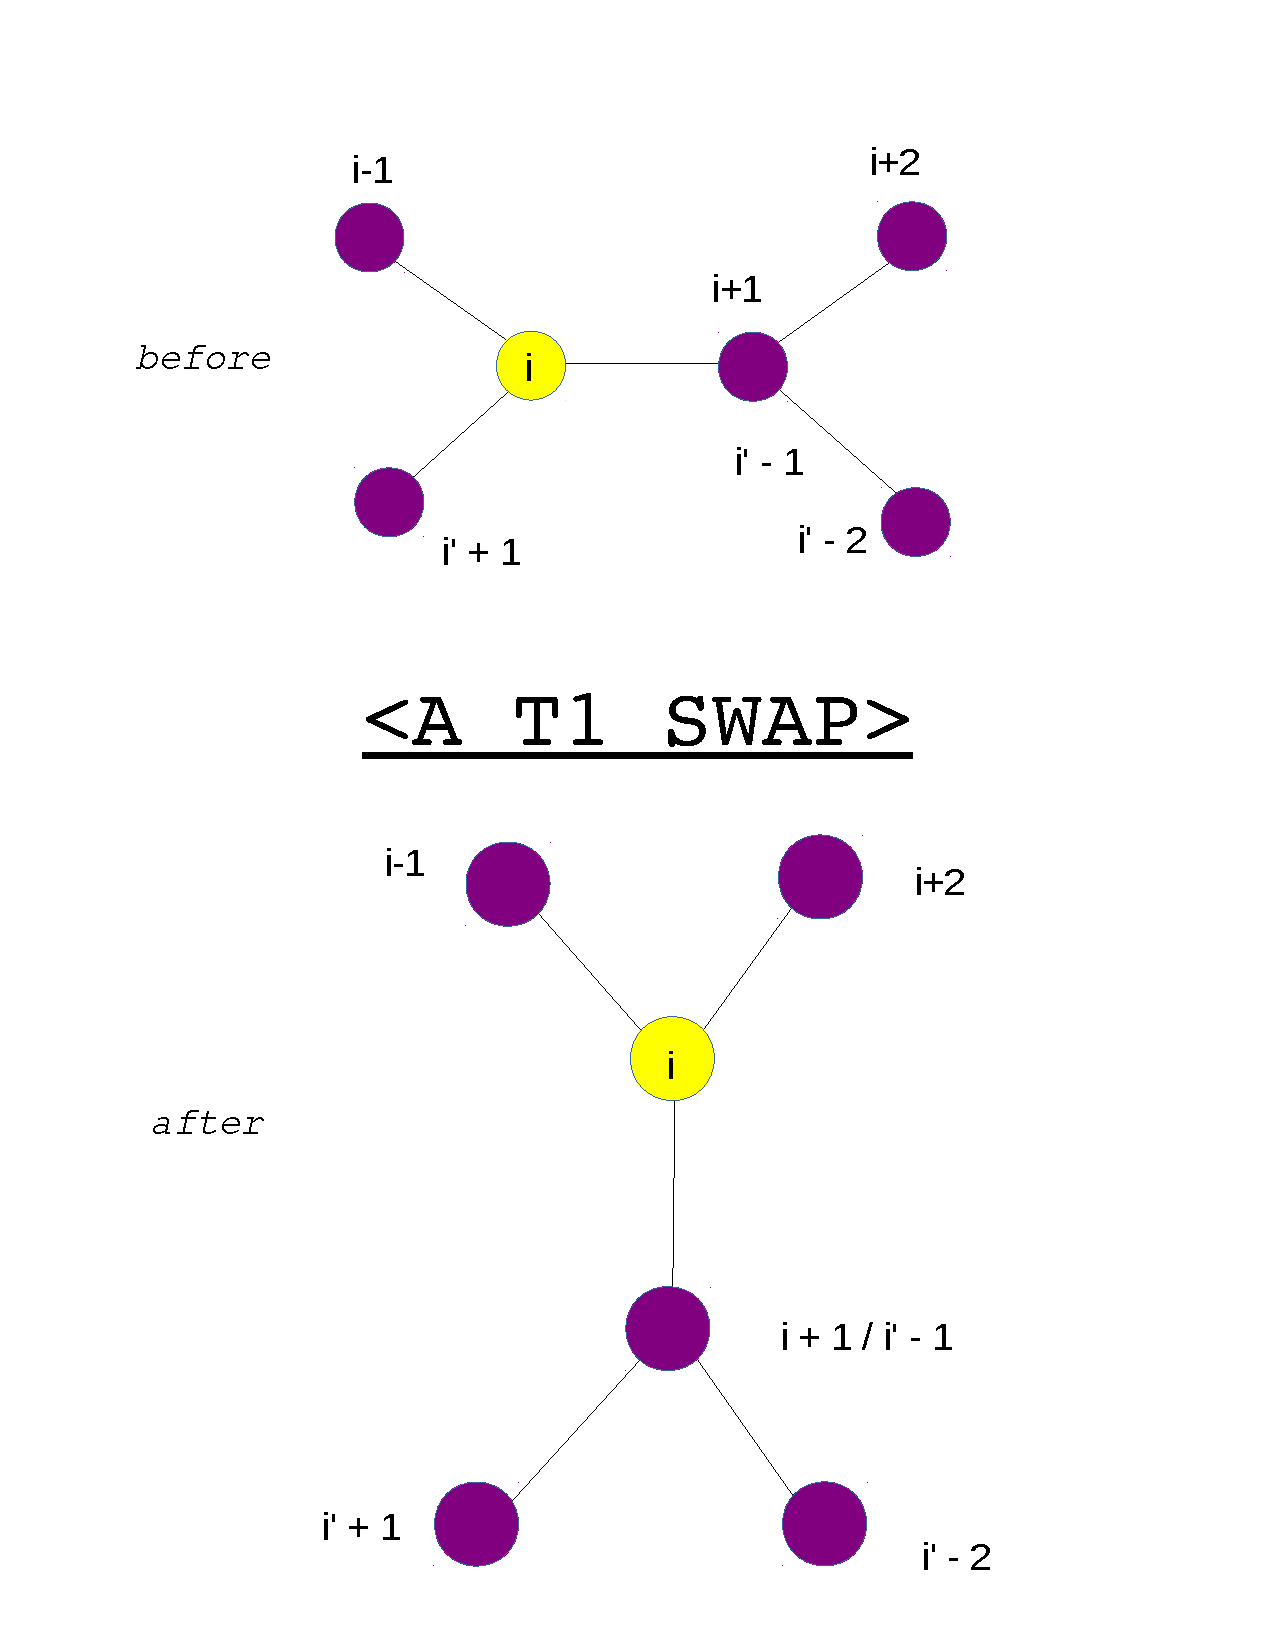
\includegraphics[width=\textwidth, height=0.8\textheight, keepaspectratio]{../diagrams/t1.pdf}
    \label{fig:t1}
    \caption[A T1 Swap]{A T1 Swap. The numbers reflect the counterclockwise storage of the vertices. The prime serves to distinguish an index in the top cell from an index in the bottom cell.}
\end{figure}
There is emprirical evidence that nearly all vertices in a sheet of epithelial tissue have degree three. Since the coordination number of the almost all vertices is three, this has led many modelers to consider what sort of topological changes can occur in mesh of these types of cells without changing the connectivity.  As it turns out, there are three changes which can occur.  The first is called a T1 swap and in illustrated in Figure~\ref{fig:t1}. This is also called a "neighbor exchanging swap" because, as you can see, two cells which were adjacent cease to be neighbors and two cells that weren't adjacent become neighbors. The T1 swap occurs when two vertices become critically close to each other, and instead of allowing the force to drive the vertices into each other we rotate their edge by 90 degree. In nature this sould correspond to two vertices getting very close, colliding, and then flattening out into an edge. Our model performs this action discretly as a simplifying measure, however, because otherwise for a moment a vertex would have degree four, and this would be difficult to handle with out a very complex data structure. The second topological change is the T2 swap, which is also known as the "cell removal swap." This occurs when a triangular cell becomes too small and is deleted and replaced by a single vertex. The last swap is cell division, occasionally referred to as the T3 swap. 

Cell division was not a part of the original Honda-Nagai Model, but it is now a very hot topic in computational tissue morphogenesis; it deserves mention. The challenge with implementing the T3 swap is that there are infinitely (within the bounds of floating point arithmetic) many choices about where to divide a cell, and there are several competing opinions (though no unanimouslly accepted theory) about how the dvision is oriented. Some cells divide along their longer axis, which is known as the `Hertwig's Long Axis Rule', but global tissue stress and local cell geometry are also thought to affect the orientation of cell division \cite{Order}\cite{Orientation}. The computational implementation of T3 swap is trivial, as the swap occurs by placing two new vertices in the interior of opposite edges and then connecting them by a new edge. The trouble is that it is not clear which edges ought to have vertices implanted, or where to insert these vertices, and the choice of where to divide a cell in a proliferating tissue can have profound effects upon the geometric appearance of a tissue \cite{Epithelial Topology}. There will be more discussion of cell division in the section of the paper dealing with the technical details of the implementation of \emph{Epithelium}.

\begin{figure}
\centering
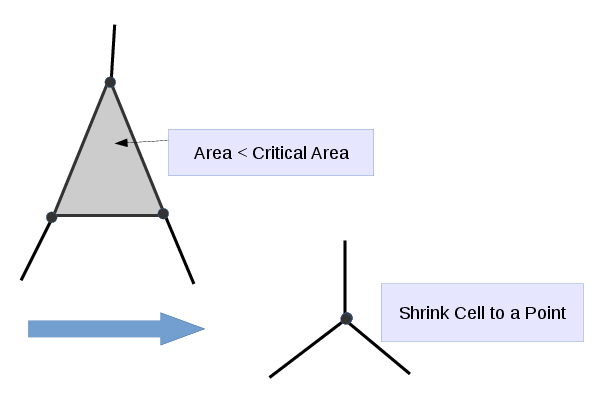
\includegraphics[width=0.5\textwidth]{../diagrams/T2swap.png}
\caption{A T2 Swap}
\label{fig:t2}
\end{figure}

\subsection{Quality, Not Quantity}

The equations in this model are dimensionless. I will not undertake a discussion of how to derive the dimensionless model from the dimensional model, but for the curious reader this is all laid out in \cite{HondaNagai}. Typically, one would not choose the values of the parameters $\alpha$, $\beta$ and $gamma$, but would instead have some dimensional biological data and go through the necessary conversion steps to convert these parameters to the simpler ones. Interestingly, in vertex dynamics literature I have read and cited in the bibliography, the only clearly stated parameters appear in \cite{ChasteMain}, and these are said to be taken from several papers which the authors (though I myself did not find these values explicity stated).  

There is little difference between equilibrium states in the Nagai-Honda model, as can be seen in the section of this paper dealing with the output of the code. Still, it has been shown that different parameter values coupled with other mesh changing operations (such as oriented cell division) can cause drastically different types of morphogenesis \cite{Overview}. For example, drosophila wings, with their highly oriented divisions, have been shown to contain approximately 80\% hexagonal cells whereas cucumber epidermis contains approximately 47\% hexagons \cite{Epithelial Topology}. While all epithelial tissue has a strong tendency towards achieving an equilibrium dominated by hexagons, the width of the distribution of cell shapes differs by cellular structure and, hence, by parameter choices \cite{Soap}. 

For those interested I have included in this paper charts which display the equilibrium meshes for different parameter values, along with a graph of the equilibrium distributions of cell sizes. These tables are found in chapter TITLE OF CHAPTER HERE. What you will see in the charts is that my implementation of the Honda-Nagai Model reproduces the results of the authors' original paper in that given a wide variety of parameterizations the mesh tends towards six sided cells. Here is one graphic from \cite{HondaNagai} in which they illustrate the distribution of cell shapes as a function of time. 

\begin{figure}
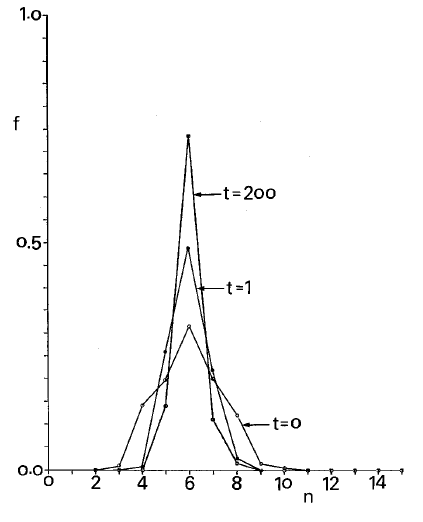
\includegraphics[width=0.5\textwidth]{../diagrams/distibutionHonda.png}
\caption{The Distribution of Cell Shapes As a Function of Time \cite{HondaNagai}}
\end{figure}
